\chapter{Conception de la Solution}

\section{Introduction}
Après avoir défini \textit{ce que} le système doit faire lors de la phase d'analyse,
la conception détermine \textit{comment} il va le faire sur le plan technique et
architectural. Ce chapitre présente l'architecture logicielle globale choisie, le cycle
de vie formalisé des incidents, la modélisation de la base de données et les diagrammes
de séquence des opérations principales.

\section{Architecture Logicielle : Modèle 3-Tiers}
Pour garantir la robustesse, la sécurité et la maintenabilité de la plateforme au sein
de l'infrastructure Naftal, nous avons adopté une \textbf{architecture à trois niveaux
(3-Tiers)}, qui est la référence des applications web d'entreprise~\cite{phpdoc}. Cette
architecture sépare logiquement l'application en trois couches indépendantes et
communicantes :

\begin{enumerate}
    \item \textbf{La couche Présentation (Frontend) :} Interface graphique rendue dans
    le navigateur web. Elle est construite avec \textbf{HTML5}, \textbf{CSS3} et le
    framework \textbf{Bootstrap~5}, et enrichie avec la librairie \textbf{DataTables}
    pour des tableaux interactifs. Elle est responsable de l'affichage et de la collecte
    des données saisies par l'utilisateur.

    \item \textbf{La couche Logique Métier (Backend) :} Gérée par le moteur
    \textbf{PHP~8} exécuté côté serveur. C'est le « cerveau » de l'application. Elle
    contient toutes les règles de gestion : vérification des sessions, contrôle des rôles
    (\texttt{requireRole()}), logique de transition des statuts, et écriture dans le journal
    d'audit. Les actions applicatives sont contenues dans des scripts dédiés
    (\texttt{actions/update\_ticket.php}, \texttt{actions/submit\_ticket.php}).

    \item \textbf{La couche Données (Base de données) :} Hébergée sur
    \textbf{Microsoft SQL Server Express}. Elle stocke de manière persistante et
    sécurisée toutes les informations. La communication entre PHP et SQL Server est
    assurée par l'extension \textbf{PDO\_SQLSRV}, qui utilise des requêtes paramétrées
    pour prévenir les injections SQL.
\end{enumerate}

\begin{figure}[H]
    \centering
     \includegraphics[width=0.75\textwidth]{figures/architecture_3tiers.png}
    \caption{Architecture 3-Tiers de la plateforme GIA}
    \label{fig:architecture}
\end{figure}

Un principe fondamental de cette architecture est que la base de données n'est
\textbf{jamais exposée directement} à l'utilisateur. Tout passe par la couche PHP,
qui joue le rôle de gardien des règles de l'organisation.

\section{Principes de sécurité et de confiance}
La conception intègre plusieurs mécanismes complémentaires, inspirés des bonnes pratiques
web classiques~\cite{phpdoc} :
\begin{itemize}
    \item \textbf{Authentification stateful :} session serveur après contrôle des identifiants ;
    expiration de session conforme à la configuration PHP.
    \item \textbf{Contrôle d'accès :} chaque page ou action sensible vérifie le rôle avant
    exécution (principe du moindre privilège).
    \item \textbf{Protection de la couche données :} utilisation de PDO avec requêtes liées ;
    jamais de concaténation directe de saisies utilisateur dans le SQL.
    \item \textbf{Traçabilité :} journal \texttt{incident\_logs} permettant une relecture
    \textit{a posteriori} des décisions et changements d'état (utile en audit interne).
    \item \textbf{Fichiers joints :} stockage hors webroot logique ou contrôle d'accès via
    l'application ; droits NTFS du compte d'exécution IIS limités au strict nécessaire.
\end{itemize}
Ces choix ne dispensent pas d'une politique de mots de passe côté annuaire ou procédures
Naftal : ils constituent la \textbf{couche applicative} du dispositif.

\section{Modélisation du Comportement : Cycle de Vie d'un Incident}
La force de notre solution réside dans la gestion \textbf{stricte et traçable} du statut
de chaque ticket. Un incident suit une machine à états (State Machine) rigoureuse dont
chaque transition est enregistrée dans le journal d'audit.

\begin{table}[H]
\centering
\begin{tabular}{@{}p{3cm}p{9cm}@{}}
\toprule
\textbf{Statut} & \textbf{Signification métier} \\ \midrule
\texttt{Ouvert} & Ticket créé ; dans la file d'attente, aucun technicien n'en est responsable. \\
\texttt{Assigné} & Un technicien est lié au ticket (\texttt{assigned\_to} renseigné). \\
\texttt{Diagnostic} & Travail en cours : analyse, investigation, correction active. \\
\texttt{Résolu} & Problème traité du point de vue technique. \\
\texttt{Clos} & Dossier fermé administrativement (date de clôture renseignée). \\
\texttt{Échec/Bloqué} & Issue finale : incident non résolvable dans les conditions prévues. \\ \bottomrule
\end{tabular}
\caption{Machine à états du cycle de vie d'un ticket d'incident}
\label{tab:lifecycle}
\end{table}

\noindent\textbf{Logique intelligente de retour en file :} Si un technicien remet un
ticket à l'état \texttt{Ouvert}, le système annule automatiquement l'assignation
(le champ \texttt{assigned\_to} est remis à NULL) et le ticket réintègre la file
d'attente globale, prêt à être pris en charge par n'importe quel technicien disponible.

\section{Modélisation de la Base de Données}

\subsection{Modèle Entité-Association (Conceptuel)}
Les relations entre les entités principales sont les suivantes~\cite{roques2006} :
\begin{itemize}
    \item Un \textbf{utilisateur} peut créer plusieurs \textbf{incidents}
    (relation 1-N via \texttt{incidents.user\_id}).
    \item Un \textbf{utilisateur} (technicien) peut être assigné à plusieurs
    \textbf{incidents} (relation 1-N via \texttt{incidents.assigned\_to}, nullable).
    \item Un \textbf{incident} possède plusieurs \textbf{lignes de journal}
    (relation 1-N via \texttt{incident\_logs.incident\_id}).
    \item Un \textbf{incident} peut avoir plusieurs \textbf{pièces jointes}
    (relation 1-N via \texttt{attachments.incident\_id}).
\end{itemize}

\begin{figure}[H]
    \centering
     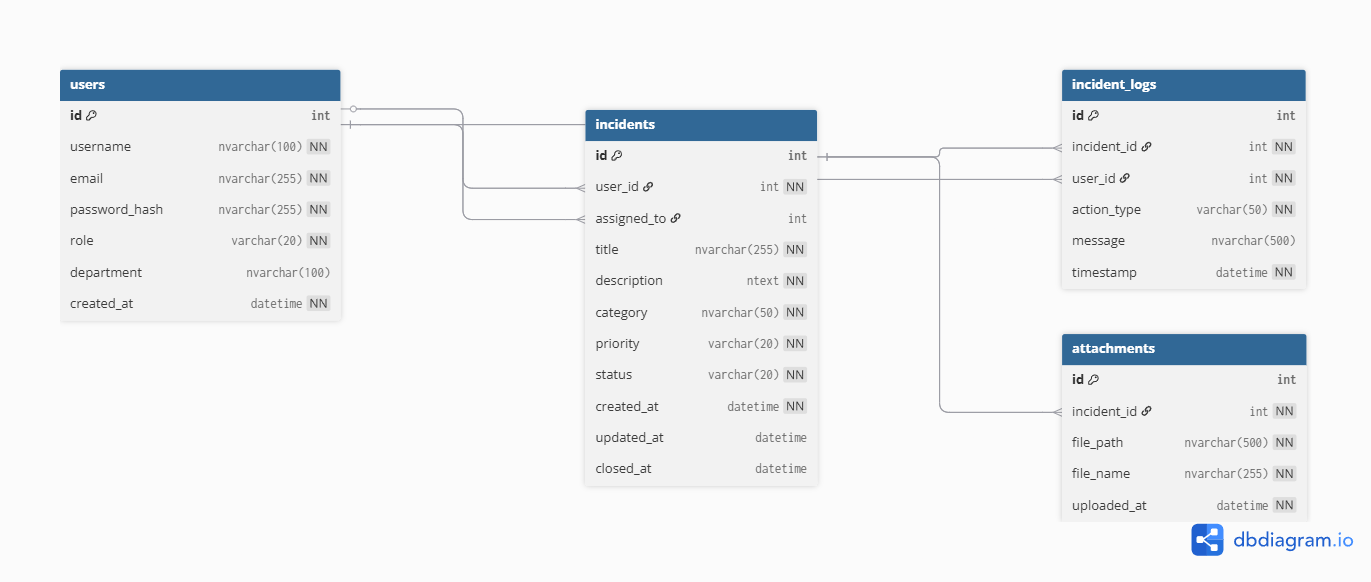
\includegraphics[width=0.85\textwidth]{figures/erd.png}
    \caption{Diagramme Entité-Association (ERD) de la base de données GIA}
    \label{fig:erd}
\end{figure}

\subsection{Dictionnaire de Données}

\begin{longtable}{@{}llp{1.4cm}p{6.2cm}@{}}
\caption{Dictionnaire de données relationnel de la base \texttt{GIA\_IncidentDB}\label{tab:datadict}} \\
\toprule
\textbf{Colonne} & \textbf{Type} & \textbf{Clé} & \textbf{Description} \\
\midrule
\endfirsthead
\multicolumn{4}{c}{\tablename\ \thetable{} — \textit{suite}} \\
\toprule
\textbf{Colonne} & \textbf{Type} & \textbf{Clé} & \textbf{Description} \\
\midrule
\endhead
\midrule
\multicolumn{4}{r}{\textit{Suite page suivante}} \\
\endfoot
\bottomrule
\endlastfoot
\multicolumn{4}{l}{\textit{Table \texttt{users} — Comptes et rôles}} \\
\midrule
\texttt{id} & INT IDENTITY & PK & Identifiant unique de l'utilisateur. \\
\texttt{username} & NVARCHAR(100) & UNIQUE & Nom de connexion. \\
\texttt{email} & NVARCHAR(255) & UNIQUE & Adresse e-mail professionnelle. \\
\texttt{password\_hash} & NVARCHAR(255) & & Mot de passe haché (jamais stocké en clair). \\
\texttt{role} & VARCHAR(20) & & Valeurs : Reporter, Technician, Admin. \\
\texttt{department} & NVARCHAR(100) & & Service ou direction d'affectation. \\
\texttt{created\_at} & DATETIME & & Date de création du compte. \\
\midrule
\multicolumn{4}{l}{\textit{Table \texttt{incidents} — Tickets d'incident}} \\
\midrule
\texttt{id} & INT IDENTITY & PK & Numéro unique du ticket. \\
\texttt{user\_id} & INT & FK$\rightarrow$\texttt{users} & Créateur (reporter). \\
\texttt{assigned\_to} & INT NULL & FK$\rightarrow$\texttt{users} & Technicien assigné ; \texttt{NULL} si en file. \\
\texttt{title} & NVARCHAR(255) & & Titre synthétique du problème. \\
\texttt{description} & NTEXT & & Description détaillée et contexte. \\
\texttt{category} & NVARCHAR(50) & & Catégorie applicative ou métier. \\
\texttt{priority} & VARCHAR(20) & & Critical, Major, Minor (niveau d'urgence). \\
\texttt{status} & VARCHAR(20) & & Statut dans la machine à états (Open, Assigned, etc.). \\
\texttt{created\_at} & DATETIME & & Date et heure de création. \\
\texttt{updated\_at} & DATETIME NULL & & Dernière modification (mise à jour automatique possible). \\
\texttt{closed\_at} & DATETIME NULL & & Date de clôture administrative si applicable. \\
\midrule
\multicolumn{4}{l}{\textit{Table \texttt{incident\_logs} — Journal d'audit}} \\
\midrule
\texttt{id} & INT IDENTITY & PK & Identifiant de la ligne de journal. \\
\texttt{incident\_id} & INT & FK$\rightarrow$\texttt{incidents} & Ticket concerné. \\
\texttt{user\_id} & INT & FK$\rightarrow$\texttt{users} & Auteur de l'action. \\
\texttt{action\_type} & VARCHAR(50) & & Ex.\ Creation, Assignment, Status Change. \\
\texttt{message} & NVARCHAR(500) NULL & & Détail lisible de l'événement. \\
\texttt{timestamp} & DATETIME & & Horodatage serveur de l'événement. \\
\midrule
\multicolumn{4}{l}{\textit{Table \texttt{attachments} — Fichiers joints}} \\
\midrule
\texttt{id} & INT IDENTITY & PK & Identifiant du fichier. \\
\texttt{incident\_id} & INT & FK$\rightarrow$\texttt{incidents} & Ticket parent. \\
\texttt{file\_path} & NVARCHAR(500) & & Chemin physique sur le serveur. \\
\texttt{file\_name} & NVARCHAR(255) & & Nom affiché à l'utilisateur. \\
\texttt{uploaded\_at} & DATETIME & & Date et heure d'envoi. \\
\end{longtable}

\begin{figure}[H]
    \centering
    % Chemin vers votre image (assurez-vous d'avoir enregistré l'image générée dans ce dossier)
    \includegraphics[width=0.95\textwidth]{figures/dictionnaire_donnees_gia.png}
    \caption{Schéma graphique du dictionnaire de données et des relations (GIA\_IncidentDB)}
    \label{fig:datadict_visual}
\end{figure}

\subsection{Commentaire entité par entité}
\textbf{Table \texttt{users}.} Elle centralise l'authentification et le profil minimal (nom,
e-mail, rôle, service). Les clés uniques sur \texttt{username} et \texttt{email} évitent les
doublons de compte. Le rôle est une énumération contrôlée côté application (Reporter, Technician,
Admin).

\textbf{Table \texttt{incidents}.} C'est l'agrégat métier principal : titre, description riche,
catégorie, priorité, statut, liens vers créateur (\texttt{user\_id}) et technicien
(\texttt{assigned\_to}, nullable). Les dates \texttt{created\_at}, \texttt{updated\_at} et
\texttt{closed\_at} permettent des indicateurs de délai (temps avant première prise en charge,
durée de résolution). La cohérence statut / assignation est assurée par la logique PHP (retour
\texttt{Ouvert} $\rightarrow$ \texttt{assigned\_to} nul).

\textbf{Table \texttt{incident\_logs}.} Elle matérialise la mémoire immuable du parcours du
ticket : type d'action, message, auteur, horodatage. Même si l'écran courant d'un incident ne
montre qu'un sous-ensemble, la table conserve l'intégralité des événements — ce qui distingue un
outil de support «\,traçable\,» d'une simple liste modifiable.

\textbf{Table \texttt{attachments}.} Elle référence les fichiers stockés sur le serveur (chemin
physique, nom d'affichage). La suppression d'un ticket peut être assortie d'une politique de
rétention des fichiers (hors périmètre fonctionnel initial mais à prévoir en exploitation).

\subsection{Intégrité référentielle et cardinalités}
Toute ligne de \texttt{incidents} référence un utilisateur existant comme créateur ; le
technicien assigné, s'il est renseigné, doit exister dans \texttt{users}. Les lignes de
\texttt{incident\_logs} et \texttt{attachments} référencent un \texttt{incident\_id} valide.
En cas de suppression d'un utilisateur (opération rare, réservée à l'admin), la stratégie peut
être le soft-delete ou la réaffectation des clés étrangères — choix d'exploitation documenté
pour éviter les orphelins.

\subsection{Indexation et performances}
Pour les filtres courants (file d'attente : statut \texttt{Ouvert} et \texttt{assigned\_to}
\texttt{NULL} ; vues technicien : \texttt{assigned\_to} = id courant), des index non clusters sur
(\texttt{status}, \texttt{assigned\_to}) et sur \texttt{created\_at} accélèrent les requêtes. Les
KPIs administrateur s'appuient sur des agrégations ; sur des volumes importants, des vues
indexées ou des snapshots périodiques pourraient être ajoutés.

% -----------------------------------------------
\section{Modélisation Mérise : MCD et MLD}
% -----------------------------------------------

\subsection{Modèle Conceptuel de Données (MCD)}

\begin{figure}[H]
  \centering
  \includegraphics[width=0.92\textwidth]{figures/mcd_gia}
  \caption[MCD de la base GIA\_IncidentDB]{Modèle Conceptuel de Données (MCD) —
           base \texttt{GIA\_IncidentDB}}
  \label{fig:mcd_gia}
\end{figure}

\paragraph{Lecture du MCD}
Un \textbf{Utilisateur} crée un ou plusieurs incidents
(1,1\,--\,0,N) ; un technicien peut en traiter plusieurs
(0,N\,--\,0,1). Chaque incident appartient à une seule
\textbf{Catégorie}, génère des entrées dans
\textbf{INCIDENT\_LOGS} (traçabilité) et peut recevoir
des \textbf{Pièces jointes}.

% -----------------------------------------------
\subsection{Modèle Logique de Données (MLD)}
% -----------------------------------------------

Le MLD est dérivé du MCD par application des règles
de passage Mérise : la clé du côté cardinalité~1 migre
vers la table côté~N comme clé étrangère~(\#).

\begin{itemize}
  \item \textbf{UTILISATEURS}(\underline{id}, username,
        email, password\_hash, rôle, département,
        date\_création)\\
        \textit{Contraintes :} \texttt{username} UNIQUE ;
        \texttt{email} UNIQUE ;
        rôle $\in$ \{Reporter, Technician, Admin\}

  \item \textbf{INCIDENTS}(\underline{id}, titre,
        description,
        catégorie\_id\textsuperscript{\#},
        priorité, statut,
        user\_id\textsuperscript{\#},
        assigned\_to\textsuperscript{\#},
        date\_création, date\_màj, date\_clôture)\\
        \textit{Clés étrangères :}
        \texttt{user\_id}~$\rightarrow$~UTILISATEURS(id) ;
        \texttt{assigned\_to}~$\rightarrow$~UTILISATEURS(id) ;
        \texttt{catégorie\_id}~$\rightarrow$~CATÉGORIES(id)\\
        \textit{Contrainte :}
        statut $\in$ \{Ouvert, Assigné, Diagnostic,
        Résolu, Clos, Bloqué\}

  \item \textbf{CATÉGORIES}(\underline{id}, libellé,
        description)\\
        \textit{Contrainte :} \texttt{libellé} UNIQUE

  \item \textbf{INCIDENT\_LOGS}(\underline{id},
        incident\_id\textsuperscript{\#},
        user\_id\textsuperscript{\#},
        type\_action, message, horodatage)\\
        \textit{Remarque :} table en écriture seule
        (journal d'audit immuable)

  \item \textbf{PIÈCES\_JOINTES}(\underline{id},
        incident\_id\textsuperscript{\#},
        chemin\_fichier, nom\_affichage, date\_envoi)
\end{itemize}

\paragraph{Règles d'intégrité applicative}
\begin{enumerate}
  \item[\textbf{R1}] Suppression en cascade :
        \texttt{INCIDENTS}~$\rightarrow$~\texttt{INCIDENT\_LOGS}
        et \texttt{PIÈCES\_JOINTES}
        (\texttt{ON DELETE CASCADE}).
  \item[\textbf{R2}] Si le statut revient à
        \texttt{Ouvert}, alors
        \texttt{assigned\_to}~$=$~\texttt{NULL}.
  \item[\textbf{R3}] Toute transition de statut génère
        obligatoirement une entrée dans
        \texttt{INCIDENT\_LOGS}.
\end{enumerate}

\section{Projection des cas d'utilisation sur les composants logiciels}
Le tableau~\ref{tab:corresp_uc} relie les principaux cas d'utilisation aux artefacts de
l'implémentation (fichiers indicatifs — noms alignés sur le dépôt du projet).

\begin{table}[H]
\centering
\small
\begin{tabular}{@{}p{4.5cm}p{10.5cm}@{}}
\toprule
\textbf{Cas d'utilisation (extrait)} & \textbf{Composants} \\
\midrule
S'authentifier & Script login, vérification session, pages protégées par \texttt{requireRole()}. \\
Créer un ticket & Formulaire HTML, \texttt{submit\_ticket.php}, INSERT \texttt{incidents/logs}. \\
Consulter la file & Liste DataTables, requêtes SQL filtrées, vues Technicien. \\
S'assigner & Action dédiée, UPDATE \texttt{assigned\_to}, log \texttt{Assignment}. \\
Changer statut & \texttt{update\_ticket.php}, validation transitions, log. \\
Voir KPIs admin & Requêtes agrégées, cartes Bootstrap, dashboard administrateur. \\
\bottomrule
\end{tabular}
\caption{Correspondance cas d'utilisation — composants}
\label{tab:corresp_uc}
\end{table}

\section{Conclusion}
La phase de conception a abouti à une architecture 3-Tiers claire, une machine à
états rigoureuse pour le cycle de vie des tickets, et un modèle de base de données
relationnel garantissant l'intégrité et la traçabilité complète des données. Ces
fondations solides ont guidé l'ensemble de la phase de réalisation.
